\documentclass{if-beamer}

\title[]{Badass Title}
\subtitle{}
\author{Isaac Ashton, Joseph Ingenito, Peter Tonuzi}
\institute[]{The College of New Jersey}
\date{}
\logo{

\includegraphics[scale=0.10]{tcnj-logotype-400-200.jpg}
}
\subject{MAT 229, Spring 2020} % metadata
\usepackage{animate}

\graphicspath{{Images/}}
\usepackage{movie15}
\newcommand{\R}{\mathbb{R}}
\newcommand{\SL}{\mathcal{L}}
\newcommand{\Om}{\Omega}
\newcommand{\W}{\mathcal{W}}
\DeclareMathAlphabet{\mathpzc}{OT1}{pzc}{m}{it}
\newcommand{\p}{\mathpzc{p}}
\newcommand{\q}{\mathpzc{q}}
\newcommand{\z}{\mathpzc{z}}
\begin{document}

\begin{frame}
  \titlepage
\end{frame}



\begin{frame}{What is a Fractal String}

\begin{definition}
A {\bf fractal string} $\Om$ is a bounded open subset of the real line.
\end{definition}

\pause
\vspace{.2 in}

$\Omega = \displaystyle\bigcup_{j = 1}^\infty \ell_j$,\qquad $\displaystyle \SL = \text{Vol}_1\left(\Omega\right) = \sum_{j = 1}^\infty \ell_j \implies \lim_{j \to \infty} \ell_j = 0$.

\pause
\vspace{.2 in}

$\ell_1 \geq \ell_2 \geq \ell_3 \geq \cdots \geq 0$

\pause
\vspace{.2 in}

The fractal string we studied the most in particular is the {\bf Cantor String}

\end{frame}



\begin{frame}{Cantor String}
	\begin{center}
		\animategraphics[loop,controls,width=7cm]{10}{Images/CantorStringPNG/CantorStringPNG-}{0}{60}
	\end{center}
\end{frame}



\begin{frame}{Inner-Tubular Neighborhood}

\begin{definition}
{\bf Inner-tubular neighborhood}:\quad $V(\epsilon) = \text{vol}_1\{x \in \Omega\ |\ d(x,\partial\Omega) < \epsilon\}$
\end{definition}

\pause
\vspace{.2 in}

{\bf Counting function}:$\displaystyle \quad N_{\Omega}(x) = \sum_{\ell_j^{-1} \leq x}1$

\vspace{.2 in}

{\bf More Notation}: $\displaystyle \quad \W_\Om(x) = \sum_{j:\ell_j^{-1} > x}{\ell_j}$

\vspace{.2 in}

{\bf Now we can write}: $V(\epsilon) = 2\epsilon \cdot N_\Om\left(2\epsilon\right) + \W_\Om\left(2\epsilon\right)$

\end{frame}



\begin{frame}{Cantor String Volume}
	\begin{center}
		\animategraphics[loop,controls,width=7cm]{10}{Images/CantorStringVolumePNG/CantorStringVolumePNG-}{0}{60}
	\end{center}
\end{frame}



\begin{frame}{Inner Minkowski Dimension of a Fractal String}

\begin{definition}
{\bf Dimension of $\Om$}: $D_\Om =\text{inf}\left\{ \alpha \geq 0\ |\ V(\epsilon)=O\left(\epsilon^{1-\alpha}\right) \text{as  } \epsilon \rightarrow 0^{+}\right\}$
\end{definition}

\pause
\vspace{.2 in}

{\bf In other terms}: $D_\Om = \text{the smallest  }\alpha \text{ st } \displaystyle \lim_{\epsilon \to 0^{+}} \frac{V(\epsilon)}{\epsilon^{1-\alpha}}=c, \ c\in \mathbb{R}$

\pause
\vspace{.2 in}

{\bf Cantor String Dimension}: $D_{cs} = \log_3 2$

\end{frame}



%begin Peter's part
\begin{frame}{3 Dimensional Fractal Objects}

        \begin{figure}
            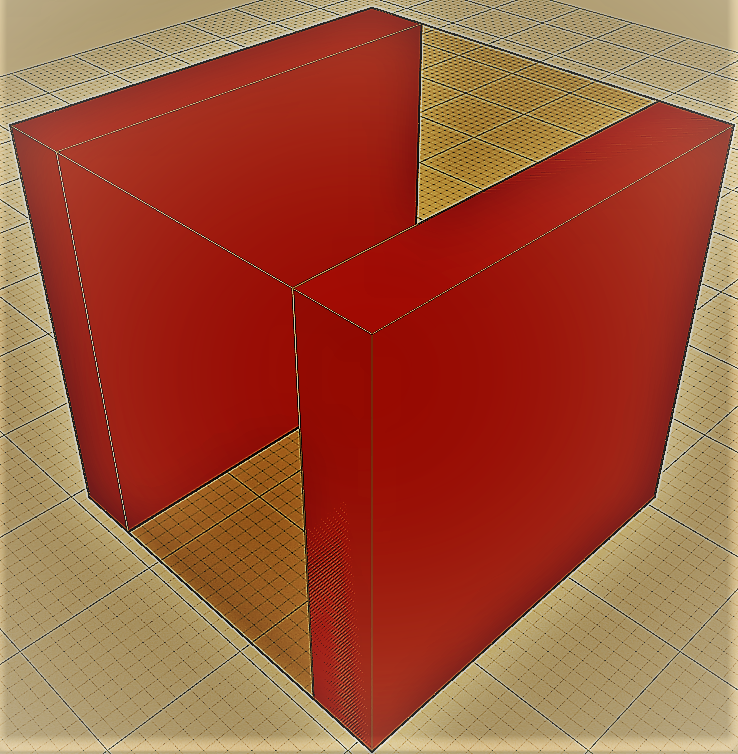
\includegraphics[height=2cm,width=2cm]{3dfractal_1.png}
            \hfill
            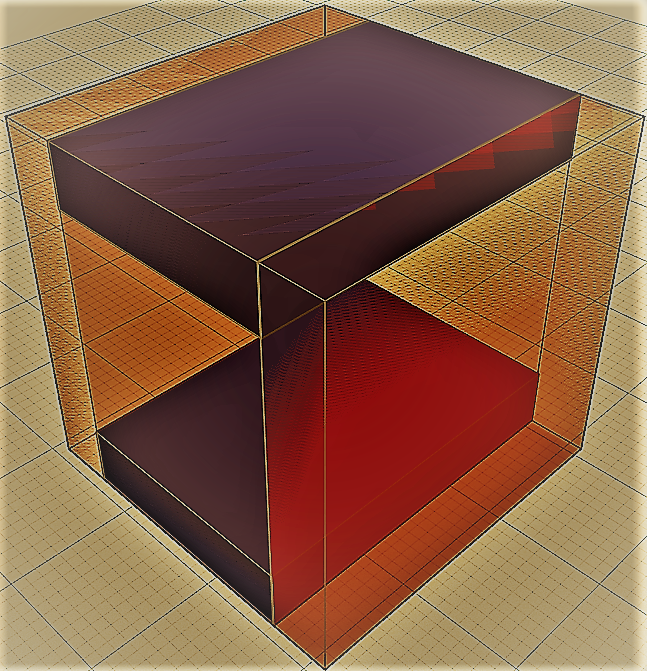
\includegraphics[height=2cm,width=2cm]{3dfractal_2.png}
            \hfill
            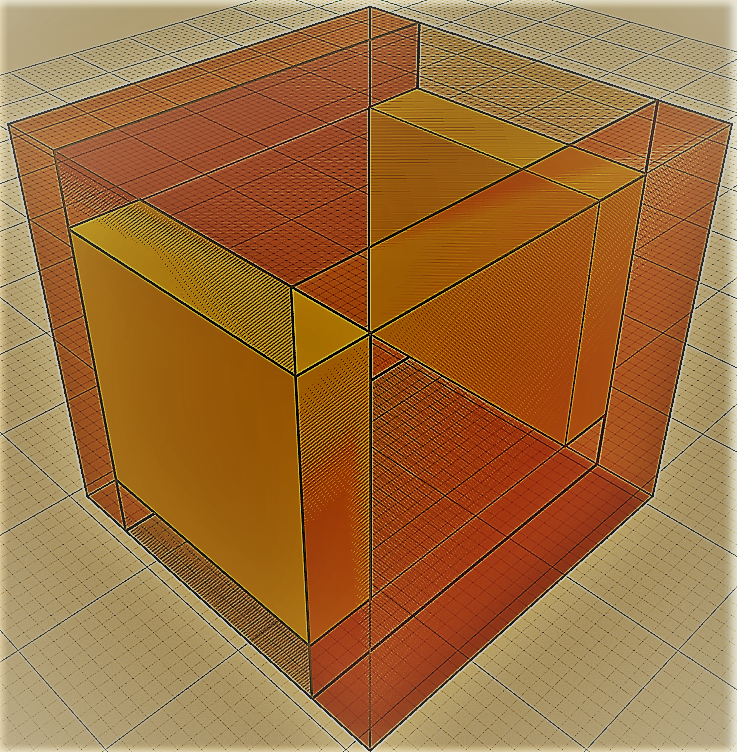
\includegraphics[height=2cm,width=2cm]{3dfractal_3.png}
            \hfill
            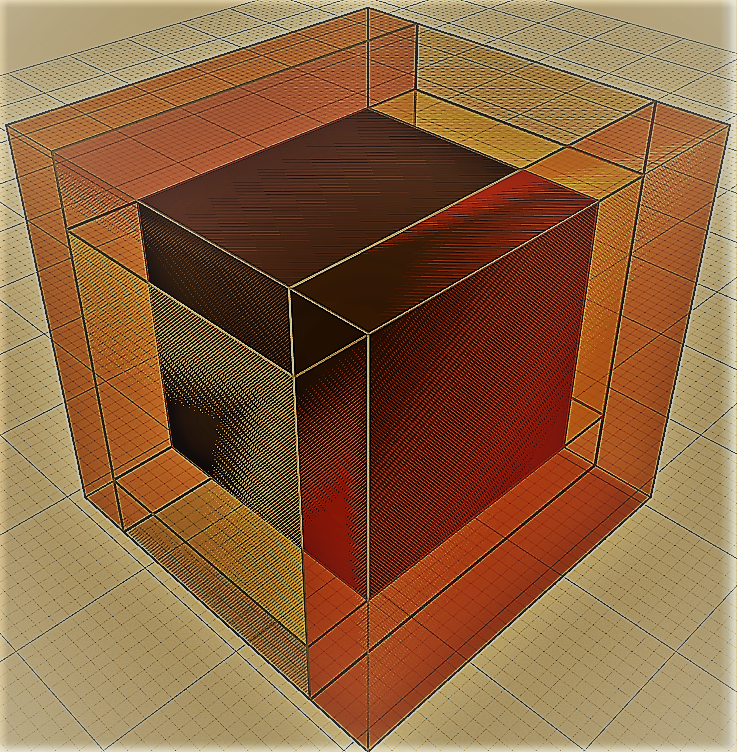
\includegraphics[height=2cm,width=2cm]{3dfractal_4.png}
            \hfill
            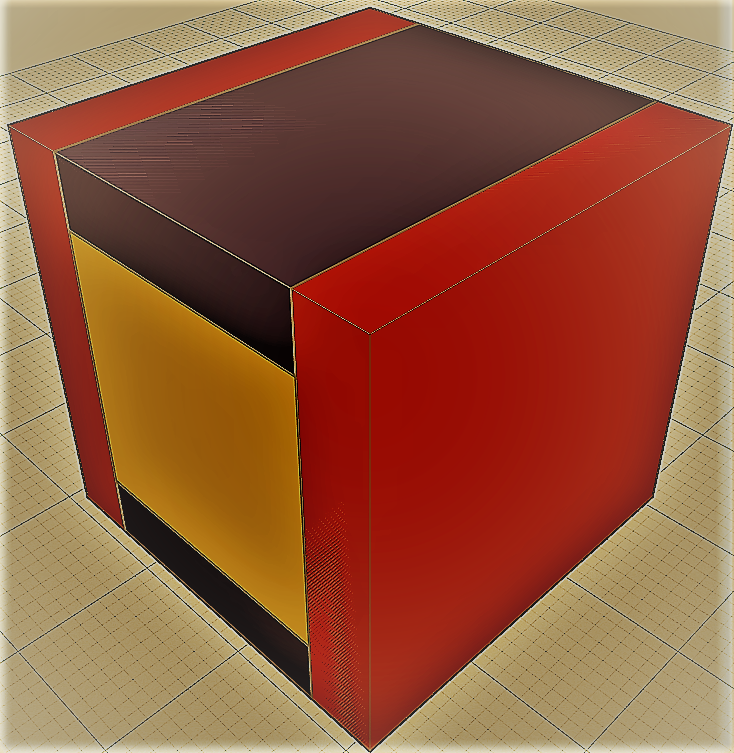
\includegraphics[height=2cm,width=2cm]{3dfractal_5}
        \end{figure}
        
        \begin{align*}
V(\epsilon) &= \textcolor{red}{2\epsilon\cdot N_{\Omega_1}(2\epsilon) \cdot \left( \sum\nolimits_{j=1}^{{N_{\Omega_2}}(2\epsilon)}\p_j \right) \cdot \left( \sum\nolimits_{j=1}^{{N_{\Omega_3}}(2\epsilon)}\q_j \right)} +\\
 &\textcolor{blue}{2\epsilon\cdot N_{\Omega_2}(2\epsilon) \cdot \left( \sum\nolimits_{j=1}^{{N_{\Omega_1}}(2\epsilon)}\ell_j - 2\epsilon \right) \cdot \left( \sum\nolimits_{j=1}^{{N_{\Omega_3}}(2\epsilon)}\q_j \right)} + \\
&\textcolor{yellow}{2\epsilon\cdot N_{\Omega_3}(2\epsilon) \cdot \left( \sum\nolimits_{j=1}^{{N_{\Omega_2}}(2\epsilon)}\p_j - 2\epsilon \right) \cdot \left( \sum\nolimits_{j=1}^{{N_{\Omega_1}}(2\epsilon)}\ell_j - 2\epsilon \right)} + \\
&\W_1\SL_2\SL_3 + \SL_1\W_2\SL_3 + \SL_1\SL_2\W_3 - \SL_1\W_2\W_3 - \W_1\SL_2\W_3 - \\
&\W_1\W_2\SL_3 + \W_1\W_2\W_3 
	\end{align*}
	
\end{frame}

\begin{frame}{3 Dimensional Fractal Volume}
$V(\epsilon) = 2\epsilon \cdot N_{\Omega_1}\cdot(\SL_2-\W_3)\cdot(\SL_3-\W_3) + 2\epsilon \cdot N_{\Omega_2}\cdot(\SL_1-\W_1-2\epsilon\cdot N_{\Omega_1})\cdot(\SL_3-\W_3) + 2\epsilon \cdot N_{\Omega_3}\cdot(\SL_2-\W_2-2\epsilon\cdot N_{\Omega_2})\cdot(\SL_1-\W_1-2\epsilon\cdot N_{\Omega_1}) + \W_1\SL_2\SL_3 + \SL_1\W_2\SL_3 + \SL_1\SL_2\W_3 - \SL_1\W_2\W_3 - \W_1\SL_2\W_3 - \W_1\W_2\SL_3 + \W_1\W_2\W_3$

\pause
\vspace{.2in}

$V(\epsilon) = \SL_1\SL_2V_3(\epsilon) + \SL_1V_2(\epsilon)\SL_3 + V_1(\epsilon)\SL_2\SL_3 - V_1(\epsilon)V_2(\epsilon)\SL_3 - V_1(\epsilon)\SL_2V_3(\epsilon)-\SL_1V_2(\epsilon)V_3(\epsilon) + V_1(\epsilon)V_2(\epsilon)V_3(\epsilon)$
\end{frame}

\begin{frame}{4 Dimensional Fractal Objects}
$V(\epsilon) = 2\epsilon\cdot N_{\Omega_1}(2\epsilon) \cdot \left( \sum_{j=1}^{{N_{\Omega_2}}(2\epsilon)}\p_j \right) \cdot \left( \sum_{j=1}^{{N_{\Omega_3}}(2\epsilon)}\q_j \right) \cdot \left( \sum_{j=1}^{{N_{\Omega_4}}(2\epsilon)}\z_j \right) + 2\epsilon\cdot N_{\Omega_2}(2\epsilon) \cdot \left( \sum_{j=1}^{{N_{\Omega_1}}(2\epsilon)}\ell_j - 2\epsilon \right) \cdot \left( \sum_{j=1}^{{N_{\Omega_3}}(2\epsilon)}\q_j \right) \cdot \left( \sum_{j=1}^{{N_{\Omega_4}}(2\epsilon)}\z_j \right) + 2\epsilon\cdot N_{\Omega_3}(2\epsilon) \cdot \left( \sum_{j=1}^{{N_{\Omega_2}}(2\epsilon)}\p_j - 2\epsilon \right) \cdot \left( \sum_{j=1}^{{N_{\Omega_1}}(2\epsilon)}\ell_j - 2\epsilon \right) \cdot \left( \sum_{j=1}^{{N_{\Omega_4}}(2\epsilon)}\z_j \right) + 2\epsilon\cdot N_{\Omega_4}(2\epsilon) \cdot \left( \sum_{j=1}^{{N_{\Omega_2}}(2\epsilon)}\p_j - 2\epsilon \right) \cdot \left( \sum_{j=1}^{{N_{\Omega_1}}(2\epsilon)}\ell_j - 2\epsilon \right) \cdot \left( \sum_{j=1}^{{N_{\Omega_3}}(2\epsilon)}\q_j - 2\epsilon \right) + \W_1\SL_2\SL_3\SL_4 + \SL_1\W_2\SL_3\SL_4 + \SL_1\SL_2\W_3\SL_4 + \SL_1\SL_2\SL_3\W_4 - \SL_1\SL_2\W_3\W_4 - \SL_1\W_2\SL_3\W_4 - \SL_1\W_2\W_3\SL_4 - \W_1\SL_2\SL_3\W_4 - \W_1\SL_2\W_3\SL_4 - \W_1\W_2\SL_3\SL_4 + \SL_1\W_2\W_3\W_4 + \W_1\SL_2\W_3\W_4 + \W_1\W_2\SL_3\W_4 + \W_1\W_2\W_3\SL_4 - \W_1\W_2\W_3\W_4$
\end{frame}

\begin{frame}{4 Dimensional Volume Formula}
$V^4(\epsilon) = \SL_1\SL_2\SL_3V_4(\epsilon) + \SL_1\SL_2V_3(\epsilon)\SL_4 + \SL_1V_2(\epsilon)\SL_3\SL_4 + V_1(\epsilon)\SL_2\SL_3\SL_4 - V_1(\epsilon)V_2(\epsilon)\SL_3\SL_4 - V_1(\epsilon)\SL_2V_3(\epsilon)\SL_4 - V_1(\epsilon)\SL_2\SL_3V_4(\epsilon) - \SL_1V_2(\epsilon)V_3(\epsilon)\SL_4 - \SL_1V_2(\epsilon)\SL_3V_4(\epsilon) - \SL_1\SL_2V_3(\epsilon)V_4(\epsilon) + V_1(\epsilon)V_2(\epsilon)V_3(\epsilon)\SL_4 + V_1(\epsilon)V_2(\epsilon)\SL_3V_4(\epsilon) + V_1(\epsilon)\SL_2V_3(\epsilon)V_4(\epsilon) + \SL_1V_2(\epsilon)V_3(\epsilon)V_4(\epsilon) -  V_1(\epsilon)V_2(\epsilon)V_3(\epsilon)V_4(\epsilon)$

\pause
\vspace{.2in}

$V^3(\epsilon) = \SL_1\SL_2V_3(\epsilon) + \SL_1V_2(\epsilon)\SL_3 + V_1(\epsilon)\SL_2\SL_3 - V_1(\epsilon)V_2(\epsilon)\SL_3 - V_1(\epsilon)\SL_2V_3(\epsilon)-\SL_1V_2(\epsilon)V_3(\epsilon) + V_1(\epsilon)V_2(\epsilon)V_3(\epsilon)$

\vspace{.2in}

$V^2(\epsilon) = \SL_1V_2(\epsilon) + V_1(\epsilon)\SL_2 - V_1(\epsilon)V_2(\epsilon)$

\end{frame}

\begin{frame}{Algebraic Manipulations}
$V^2(\epsilon) = \SL_1V_2(\epsilon) + V_1(\epsilon)\SL_2 - V_1(\epsilon)V_2(\epsilon)$
$$= (-1)\cdot(V_1(\epsilon)-\SL_1)\cdot(V_2(\epsilon)-\SL_2) + \SL_1\SL_2$$

\pause
\vspace{.2in}

$V^3(\epsilon) = \SL_1\SL_2V_3(\epsilon) + \SL_1V_2(\epsilon)\SL_3 + V_1(\epsilon)\SL_2\SL_3 - V_1(\epsilon)V_2(\epsilon)\SL_3 - V_1(\epsilon)\SL_2V_3(\epsilon)-\SL_1V_2(\epsilon)V_3(\epsilon) + V_1(\epsilon)V_2(\epsilon)V_3(\epsilon)$

$$= (-1)^2\cdot(V_1(\epsilon)-\SL_1)\cdot(V_2(\epsilon)-\SL_2)\cdot(V_3(\epsilon)-\SL_3) + \SL_1\SL_2\SL_3$$

\end{frame}

\begin{frame}{Algebraic Manipulations}
$V^4(\epsilon) = \SL_1\SL_2\SL_3V_4(\epsilon) + \SL_1\SL_2V_3(\epsilon)\SL_4 + \SL_1V_2(\epsilon)\SL_3\SL_4 + V_1(\epsilon)\SL_2\SL_3\SL_4 - V_1(\epsilon)V_2(\epsilon)\SL_3\SL_4 - V_1(\epsilon)\SL_2V_3(\epsilon)\SL_4 - V_1(\epsilon)\SL_2\SL_3V_4(\epsilon) - \SL_1V_2(\epsilon)V_3(\epsilon)\SL_4 - \SL_1V_2(\epsilon)\SL_3V_4(\epsilon) - \SL_1\SL_2V_3(\epsilon)V_4(\epsilon) + V_1(\epsilon)V_2(\epsilon)V_3(\epsilon)\SL_4 + V_1(\epsilon)V_2(\epsilon)\SL_3V_4(\epsilon) + V_1(\epsilon)\SL_2V_3(\epsilon)V_4(\epsilon) + \SL_1V_2(\epsilon)V_3(\epsilon)V_4(\epsilon) -  V_1(\epsilon)V_2(\epsilon)V_3(\epsilon)V_4(\epsilon)$
$$ = (-1)^3\cdot(V_1(\epsilon)-\SL_1)\cdot(V_2(\epsilon)-\SL_2)\cdot(V_3(\epsilon)-\SL_3)\cdot(V_4(\epsilon)-\SL_4) + \SL_1\SL_2\SL_3\SL_4$$
\end{frame}

\begin{frame}{General Volume Formula}

$$V^2(\epsilon)= (-1)\cdot(V_1(\epsilon)-\SL_1)\cdot(V_2(\epsilon)-\SL_2) + \SL_1\SL_2$$

$$ V^3(\epsilon) = (-1)^2\cdot(V_1(\epsilon)-\SL_1)\cdot(V_2(\epsilon)-\SL_2)\cdot(V_3(\epsilon)-\SL_3) + \SL_1\SL_2\SL_3$$

$$ V^4(\epsilon)= (-1)^3\cdot(V_1(\epsilon)-\SL_1)\cdot(V_2(\epsilon)-\SL_2)\cdot(V_3(\epsilon)-\SL_3)\cdot(V_4(\epsilon)-\SL_4) + \SL_1\SL_2\SL_3\SL_4$$

$$V^{n}(\epsilon) =\left[ (-1)^{n-1} \cdot \displaystyle \prod_{k = 1}^{n}(V_k(\epsilon)-\SL_k)\right] +\prod_{k = 1}^{n} \SL_k$$

\end{frame}

\begin{frame}{Future Work}
\begin{itemize}

\item Prove the general volume formula

\item Find a general formula for dimension (based on general volume formula)

\end{itemize}
\end{frame}


\begin{frame}[allowframebreaks]
\frametitle{References}

\begin{thebibliography}{1}

\bibitem{bini2014solving} 
D. A. Bini and L. Robol.
``Solving secular and polynomial equations: A multiprecision algorithm.'' 
\textit{Journal of Computational and Applied Mathematics}
272
(2014),
276--292.

\bibitem{bremner2011lattice} 
M. R. Bremner.
\textit{Lattice Basis Reduction: An Introduction to the LLL Algorithm and its Applications},
Taylor \& Francis, Boca Raton, 2011.

\bibitem{lapidus1991fractal} 
M. L. Lapidus.
``Fractal drum, inverse spectral problems for elliptic operators and a partial resolution of the Weyl-Berry conjecture.'' 
\textit{Transactions of the American Mathematical Society.}
(2)
325
(1991),
465--529.
 
\bibitem{lapidus1993vibrations} 
M. L. Lapidus.
``Vibrations of Fractal Drums, the Riemann Hypothesis, Waves in Fractal Media and the Weyl-Berry Conjecture.'' In \textit{Ordinary and Partial Differential Equations}, edited by B. D. Sleeman and R. J. Jarvis, Vol. IV, Proc. Twelfth Intern. Conf. (Dundee, Scotland, UK, June 1992), Pitman Research Notes in Math. Series 289, pp. 126--209, London: Longman Scientific and Technical, 1993.

\bibitem{lapidus2008in} 
M. L. Lapidus.
\textit{In Search of the Riemann Zeros: Strings, fractal membranes and noncommutative spacetimes}, 
American Mathematical Society, Providence, Rhode Island, 2008.

\bibitem{lapidus2019an} 
M. L. Lapidus.
``An overview of the complex fractal dimensions: From fractal strings to fractal drums, and back,'' \textit{Contemporary Mathematics}, Vol. 731, Amer. Math. Soc., Providence, R.I., 2019, 143--269

\bibitem{lapidus1993the} 
M. L. Lapidus and C. Pomerance.
``The Riemann Zeta-Function and the One-Dimensional Weyl-Berry Conjecture for Fractal Drums,''
\textit{Proc. London Math. Soc.}
(3)
66
(1993),
41--69.

\bibitem{lapidus1995the} 
M. L. Lapidus and H. Maier.
``The Riemann Hypothesis and Inverse Spectral Problems for Fractal Strings.'' \textit{J. London Math. Soc.}
(2)
52
(1995),
15--34.

\bibitem{lapidus2000fractal} 
M. L. Lapidus and M. van Frankenhuijsen.
\textit{Fractal Geometry and Number Theory \textup(Complex dimensions of fractal strings and zeros of zeta functions\textup)},
Birkh\"auser, Boston, 2000.

\bibitem{lapidus2003complex}
M. L. Lapidus and M. van Frankenhuijsen.
``Complex Dimensions of Self-Similar Fractal Strings and Diophantine Approximation,''  
\textit{J. Experimental Math.}
(1)
12
(2003),
41--69. 

\bibitem{lapidus2012fractal} 
M. L. Lapidus and M. van Frankenhuijsen.
\textit{Fractal Geometry, Complex Dimensions and Zeta Functions: Geometry and Spectra of Fractal Strings}, second edition (of the 2006 edition),
Springer Monographs in Mathematics, Springer, New York, 2012.

\bibitem{lapidus2017fractal} 
M. L. Lapidus and G. Radunovi\'c and D. {\u Z}ubrini\'c.
\textit{Fractal Zeta Functions and Fractal Drums: Higher-Dimensional Theory of Complex Dimensions},
Springer Monographs in Mathematics, Springer, New York, 2017.

\bibitem{lenstra1982factoring}
A. K. Lenstra and H. W. Lenstra and L. Lov\'asz.
``Factoring polynomials with rational coefficients,''  
\textit{Mathematische Annalen}
(4)
261
(1982),
515--534. 

\bibitem{schmidt1980diophantine} 
W. M. Schmidt.
\textit{Diophantine Approximation},
Springer, New York, 1980.

\bibitem{serre1973a} 
J.-P. Serre.
\textit{A Course in Arithmetic\textup{, English translation}},
Springer-Verlag, Berlin, 1973.

\bibitem{voskanian2019on} 
E. K. Voskanian.
``On the Quasiperiodic Structure of the Complex Dimensions of Self-Similar Fractal Strings,''
Ph. D. Dissertation, University of California, Riverside, 2019.

\end{thebibliography}

\end{frame}





\end{document}
